	\section{Simulation der Transistor Matrix}
	Die Simulation der Transistor Matrix wurde f�r alle drei Leistungsangaben durchgef�hrt. Dabei wurde von dem Initial-Abstand von 2 mm der Transistoren ausgegangen. 
	
	\begin{table}[bh]
		\centering
		\caption{Temperaturen bei 2 mm Abstand}
		\begin{tabular}{p{2,5cm} l p{2.5cm}} 
			\rowcolor[gray]{.8} Leistung & Temperatur \\
			50 mW	& ca. 28,5 �C \\	
			\rowcolor[gray]{.8}	100 mW	& ca. 34,5 �C 	\\
			150 mW	& ca. 41,0 �C  	
		\end{tabular}
		\label{tab:Statische_Ergebnisse_Transistor}
	\end{table}
	
	Die Normtemperatur einer Maus betr�gt 38 �C, aus Tabelle \ref{tab:Statische_Ergebnisse_Transistor} ist  zu erkennen, dass f�r 50 mW diese Temperatur im Initial-Zustand  nicht erreicht werden kann. Dies gilt ebenfalls f�r 100 mW. F�r 150 mW muss der Abstand vergr��ert werden.
		
		\subsection{Optimierung}
		In der Aufgabenstellung wurde festgelegt, dass eine Optimierung hinsichtlich der Abst�nde zueinander erfolgen soll. Es wurde eine Optimierung durchgef�hrt, das aus den acht angesteuerten Transistoren ein Temperaturbereich entsteht der einen geringen Signifikanten Temperaturunterschied hat. Dabei wurde der Abstand zu den Pixeln, als auch auf die Leistung hin optimiert.
		\begin{center}
			\begin{minipage}[!ht]{0.48\textwidth}
				\captionsetup{type=figure}
				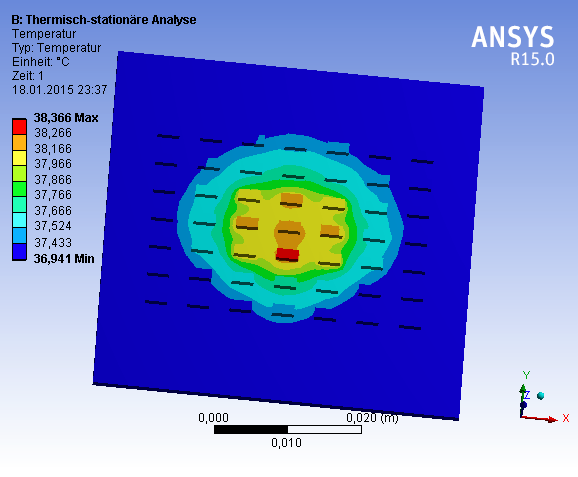
\includegraphics[width=1\linewidth]{bilder/Waermeverteilung_150mW_Transistor_Ring_innen_Kantik}
				\caption{Transistormatrix, Simulation des inneren Vierecks mit \\126 mW;\\ Max/Min Temperatur:\\ 38,366 �C / 36,941 �C}
				\label{fig:Transistor_Ringen_aussen_innen}
			\end{minipage}
			\begin{minipage}[!ht]{0.48\textwidth}
				\captionsetup{type=figure}
				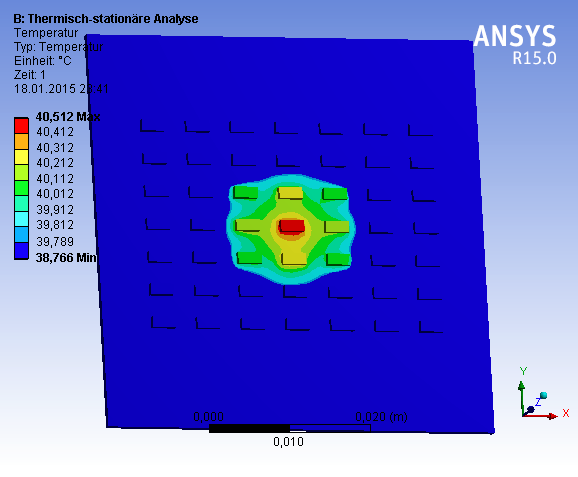
\includegraphics[width=1\linewidth]{bilder/Waermeverteilung_150mW_Transistor_grosser_Punkt_Kantik}
				\caption{Transistormatrix, Simulation der sechs inneren Pixel 126 mW;\\ Max/Min Temperatur:\\ 40,512 �C/38,766 �C}
				\label{fig:Transistor_Ringen_aussen}
			\end{minipage}
		\end{center}
		
		\subsection{Aufgabe mit Rand}
		\begin{center}
			\begin{minipage}[!ht]{0.48\textwidth}
				\captionsetup{type=figure}
				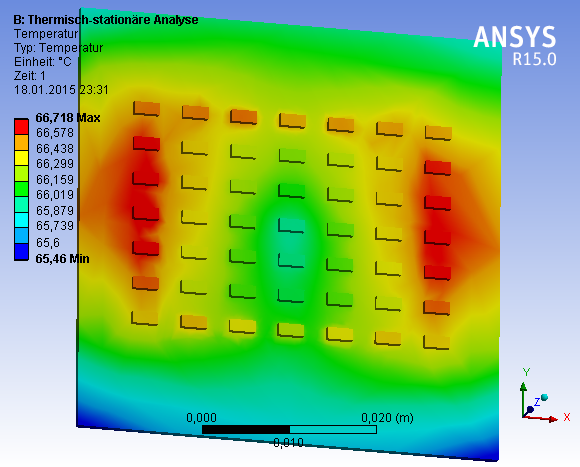
\includegraphics[width=1\linewidth]{bilder/Waermeverteilung_150mW_Transistor_Ring_aussen_Weich}
				\caption{Transistormatrix, Simulation des �u�eren Vierecks mit 150 mW;\\Max/Min Temperatur:\\ 66,718 �C/55,460 �C}
				\label{fig:Transistor_Ringen_aussen}
			\end{minipage}
			\begin{minipage}[!ht]{0.48\textwidth}
				\captionsetup{type=figure}
				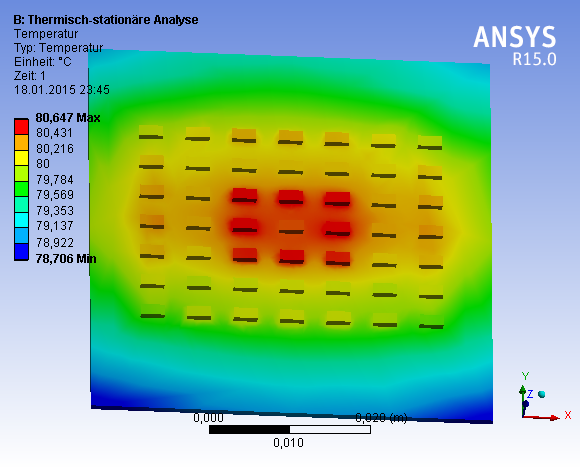
\includegraphics[width=1\linewidth]{bilder/Waermeverteilung_150mW_Transistor_Ring_aussen_innen_Weich}
				\caption{Transistormatrix, Simulation des �u�eren und inneren Vierecks mit 150 mW; \\ Max/Min Temperatur:\\ 80,647 �C/78,706 �C}
				\label{fig:Transistor_Ringen_aussen_innen}
			\end{minipage}
		\end{center}

		
		